\chapter{Contribution} % possible chapter for Projects
\label{chap:contribution}

\subsection{Data Acquisition}

IIn the Fair-by-Design workflow, the data acquisition process transcends the conventional boundaries by placing a heightened emphasis on delving into the intricacies of the data, with a particular focus on the identification and understanding of sensitive attributes. Unlike traditional data acquisition, which predominantly revolves around the collection of relevant datasets, the Fair-by-Design approach acknowledges the imperative of probing into sensitive attributes. This emphasis proves pivotal in the evaluation of fairness within the machine learning model.

The significance of comprehending these sensitive attributes cannot be overstated, given their substantial influence on the fairness of the model's outcomes. This understanding spans various dimensions, including legal considerations, ethical implications, and societal norms. Acquiring this knowledge is a nuanced process that often necessitates direct communication with stakeholders. In certain scenarios, sensitive attributes may be deliberate business choices, making engagement with stakeholders crucial for discerning the underlying motivations and expectations.

Alternatively, common-sense reasoning is applied to identify potential sensitive attributes that might impact fairness. This involves a thoughtful and context-specific analysis of the data, considering historical and societal contexts. Common-sense reasoning serves as a supplementary approach, particularly in cases where direct communication might be limited or where latent, non-obvious sensitive attributes could influence the model's outcomes.

Once the data has been acquired, and a comprehensive understanding of sensitive attributes has been obtained, the Fair-by-Design workflow advances to the next crucial step: fairness evaluation. This stage is fundamental as it lays the groundwork for subsequent model development. The fairness evaluation is meticulously designed to assess the fairness of the dataset concerning the identified sensitive attributes. This process entails quantitative analysis, statistical testing, and the application of fairness metrics, ensuring a systematic and objective evaluation of potential biases and disparities within the dataset.

By incorporating this nuanced and comprehensive approach to data acquisition and fairness evaluation, the Fair-by-Design workflow establishes a robust foundation for the development of machine learning models. These models not only meet technical performance criteria but also adhere to ethical and fairness considerations. The insights garnered from this initial phase provide valuable guidance for the subsequent stages of the workflow, contributing to the overall integrity and equity of the machine learning process.

\subsubsection{Fairness Assessment}

The fairness assessment within the Fair-by-Design workflow serves as a critical checkpoint, functioning as a meticulous examination to ascertain the absence of biases and align the dataset with ethical considerations. At this stage, the objective is to rigorously evaluate the fairness of the dataset, particularly in relation to the identified sensitive attributes. This process plays a pivotal role in establishing the ethical foundation for the subsequent stages in the machine learning pipeline.

To conduct this comprehensive evaluation, the Fair-by-Design workflow leverages Disparate Impact, a widely recognized and utilized fairness metric. Disparate Impact offers a quantitative measure of the differential treatment experienced by distinct groups within the dataset. Specifically, it assesses the ratio of favorable outcomes for various demographic groups, shedding light on potential biases and disparities that might be present.

The implementation of Disparate Impact serves as a vital indicator during the data acquisition phase, enabling practitioners to make well-informed decisions regarding fairness considerations. By quantifying the differential impact on different demographic groups, Disparate Impact facilitates a nuanced understanding of potential imbalances within the dataset, empowering practitioners to address and rectify biases before proceeding with subsequent stages of the machine learning pipeline.

The strategic integration of Disparate Impact into the fairness assessment phase underscores the commitment of the Fair-by-Design workflow to a principled and thorough approach to ensuring fairness. This metric acts as a guiding compass, steering practitioners towards fair and equitable machine learning practices from the outset of the workflow. It plays a crucial role in fostering a robust ethical foundation and promoting fairness throughout the machine learning development process.

\subsection{Data pre-processing}

The data pre-processing step within the Fair-by-Design workflow is meticulously designed as a comprehensive process that integrates both traditional and fairness-oriented sub-steps. This nuanced approach ensures the dataset's readiness for subsequent model development.

\subsubsection{Usual Pre-processing Step}

The first sub-step addresses typical operations to enhance the overall dataset quality. Handling missing values is a crucial pre-processing task, where NaN values are filled using the mean for continuous attributes and the median for discrete attributes. This standard operation ensures a more complete and standardized dataset. However, the Fair-by-Design workflow goes beyond standard pre-processing by incorporating operations specific to protected attributes and the output variable, setting the stage for defining the learning prediction goal and establishing how protected attributes should be treated.

\begin{itemize}
    
    \item \textbf{Handling Protected Attributes:} 
    
    Within the Fair-by-Design workflow, a meticulous transformation process is applied to protected attributes, assumed to be categorical in nature. This transformative step is pivotal for ensuring fairness in subsequent stages of the machine learning pipeline, aiming to mitigate potential biases associated with these attributes and foster equitable treatment within the model.

    The transformation process for categorical protected attributes involves the identification of the most frequent value and the subsequent application of a binary encoding scheme. This nuanced procedure plays a crucial role in aligning the dataset with the fairness objectives of the Fair-by-Design workflow.

    et $P$ be the set of protected attributes, and $p_i$ represent a specific protected attribute within $P$. The most frequent value, denoted as $v_{\text{freq}}$, is determined for each categorical protected attribute $p_i$ in the dataset through the following formalism:

    \[
    v_{\text{freq}} = \text{argmax}_v \left( \text{count}(p_i = v) \right)
    \]
    
    This calculation ensures a comprehensive understanding of the prevalent categories within these attributes.

    The binary representation preserves the essential information about protected attributes, providing a condensed yet informative encoding that reflects the privilege or lack thereof concerning specific attributes.

    During the training phase, the model learns to distinguish instances based on privilege or lack thereof concerning specific attributes, as represented by the binary encoding. This facilitates effective model incorporation and decision-making during training and prediction phases.

    This nuanced encoding strategy serves as the foundation for unbiased and fair treatment of instances within the model. By transforming categorical protected attributes into a binary representation, the Fair-by-Design workflow ensures that subsequent machine learning models can effectively incorporate and act upon this information during training and prediction phases, contributing significantly to the development of a more equitable and ethically sound machine learning model.

    \item \textbf{Handling Output Variable:} 
    
    The handling of the output variable in the Fair-by-Design workflow is a nuanced process that adapts to the nature of the variable, whether categorical or continuous. This tailored treatment is essential for aligning the prediction task with the fairness objectives of the workflow, ensuring that the model's predictions are not only accurate but also ethically sound.


    In cases where the output variable is categorical, the workflow initiates by determining the most frequent value within this category. Let $Y$ represent the output variable, and $y_i$ be a specific outcome within $Y$. The most frequent value, denoted as $y_{\text{freq}}$, is determined through the following formalism:

    \[
    y_{\text{freq}} = \text{argmax}_y \left( \text{count}(Y = y) \right)
    \]

    This strategic calculation provides insights into the prevailing outcome within the dataset. Subsequently, instances where the output variable matches $y_{\text{freq}}$ are replaced with the binary representation 1, while all other instances take on the binary representation 0. The binary encoding function is defined as follows:

    \[
    \text{Binary Encoding}(y_i) = \begin{cases} 
    1 & \text{if } y_i = y_{\text{freq}} \\ 
    0 & \text{otherwise}
    \end{cases}
    \]

    This transformation effectively redefines the prediction task, shifting the focus to discerning whether a given sample belongs to the most frequent outcome. The binary encoding approach not only simplifies the representation of categorical outcomes but also enables the model to make predictions in a manner that aligns with fairness considerations.


    Conversely, when the output variable is continuous, the workflow employs a distinct strategy. Let $Z$ represent the continuous output variable, and $z_i$ be a specific value within $Z$. Values of the continuous variable that surpass the mean are replaced with 1, while those falling below the mean assume the binary representation 0. This adjustment transforms the prediction task into establishing whether a sample's continuous output is above the mean. The binary encoding function for continuous variables is defined as:

    \[
    \text{Binary Encoding}(z_i) = \begin{cases} 
    1 & \text{if } z_i > \text{mean}(Z) \\ 
    0 & \text{otherwise}
    \end{cases}
    \]

    This approach ensures that the model is not only attentive to the central tendency of the continuous variable but also considers the distribution of values concerning the mean.

    This tailored and meticulous treatment of the output variable underscores the commitment of the Fair-by-Design workflow to equitable and ethical machine learning practices. The workflow not only adapts to the inherent characteristics of the data but also ensures that the subsequent model operates with a heightened awareness of fairness considerations, contributing to the development of a more responsible and unbiased machine learning model.

\end{itemize}

This nuanced pre-processing step sets the groundwork for a fair and unbiased learning prediction, aligning the dataset with the ethical considerations embedded in the Fair-by-Design workflow.

\subsubsection{Fairness pre-processing algorithms}

The second sub-step of the data pre-processing phase in the Fair-by-Design workflow is meticulously crafted to address and mitigate bias in the dataset, employing a pre-processing approach explicitly designed for fairness considerations. This phase builds upon the dataset and protected attributes obtained during the data acquisition phase, introducing three distinct algorithms strategically devised to promote fairness.

The proposed algorithms are elucidated as follows:

\begin{itemize}

    \item \emph{Fairness through Unawareness with Proxy Detection via Association Rules Mining:} This algorithm harnesses the principles of association rule mining to detect proxies within the dataset. Proxies, in this context, refer to factors that may act as intermediaries, influencing the model's predictions and potentially leading to biased outcomes. By identifying and mitigating the impact of both protected attributes and potential proxies, this algorithm aims to enhance fairness in the dataset. Detailed insights into the design, implementation, and specific fairness considerations addressed by this algorithm will be expounded upon in \cref{section:fairness}.
    
    \item \emph{Fairness through Unawareness with Proxy Detection via Variables Only:} Similar to the aforementioned approach, this algorithm focuses on averting the impact of protected attributes. However, it places specific emphasis on considering only the protected attributes during the proxy detection process. The distinctions between this approach and the association rules mining-based approach will be thoroughly delineated in \cref{section:fairness}.
    
    \item \emph{Fairness through Data Rebalancing:} In a departure from the first two approaches, which aim to mitigate the effects of specific attributes, this algorithm adopts a data rebalancing strategy. The primary goal is to render the dataset fair by proposing a novel fairness definition and redistributing the data distribution. This approach introduces a new dimension to fairness considerations, focusing on rebalancing the dataset to mitigate biases and ensure equitable representation. The intricacies of the design, implementation, and the novel fairness perspective proposed by this algorithm will be dissected in \cref{section:fairness}.

\end{itemize}

Before apply the presented algorithm or each other fairness pre-processing algorithm, the fundamental design choice at this step of the workflow is to choose the fairness metric.

The forthcoming section (\cref{section:fairness}) will provide an in-depth exploration of each algorithm, offering a comprehensive understanding of their theoretical underpinnings, practical implementation, and the specific fairness considerations they target. This detailed examination aims to equip practitioners with the insights necessary to make informed decisions about algorithm selection within the Fair-by-Design workflow.

\subsection{Performance evaluation}

After the model has undergone the training process, the evaluation phase in the Fair-by-Design workflow extends beyond traditional accuracy-based assessments. This phase places particular emphasis on incorporating fairness metrics to comprehensively evaluate the model's performance and rigorously assess the fairness of the entire workflow.

In the realm of fairness assessment, two key metrics, namely \emph{Equalized Odds} and \emph{Demographic Parity}, play a pivotal role in quantifying and analyzing the fairness implications of the model's predictions:

\begin{itemize}

    \item \emph{Equalized Odds:} This metric is designed to ensure parity in the true positive rate and false positive rate across different demographic groups. Mathematically, it involves minimizing the disparities in error rates between various subgroups. By focusing on achieving equity in both the benefits (true positives) and errors (false positives) of the model for diverse demographic groups, Equalized Odds offers a nuanced perspective on fairness. It provides a more granular understanding of how the model performs across different segments of the population, allowing practitioners to identify and rectify potential biases in prediction outcomes.
    
    \item \emph{Demographic Parity:} Demographic Parity is a fundamental fairness metric that mandates the proportion of positive outcomes to be the same for all demographic groups, irrespective of the protected attributes. This metric serves as a cornerstone for evaluating the overall fairness in the distribution of positive outcomes. It ensures that the model does not disproportionately favor or disadvantage specific demographic groups, contributing to a more unbiased and equitable evaluation of the model's performance. Demographic Parity provides valuable insights into the distributional aspects of the model's predictions and aids in uncovering any systemic disparities in positive outcome rates among different subgroups.

\end{itemize}
The integration of these advanced fairness metrics in the evaluation process enhances the transparency and ethical considerations of the Fair-by-Design workflow. Beyond traditional accuracy metrics, these fairness metrics offer a more nuanced understanding of how the model impacts different demographic groups, promoting a comprehensive evaluation of fairness implications. The upcoming sections will delve into a detailed analysis of the results obtained through the application of these metrics, providing deeper insights into the fairness considerations of the developed machine learning model.

Here's the graphical representation of the presented workflow:

\begin{center}

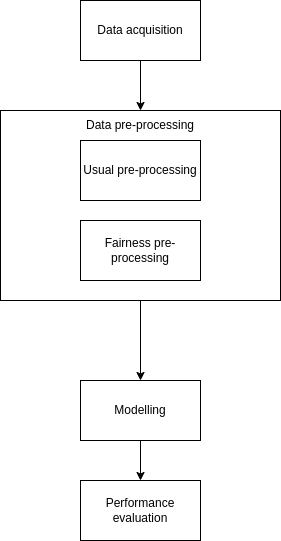
\includegraphics[width=.5\textwidth, height=1.0\textwidth]{fairness-workflow.png}

\end{center}

\newpage
\section{Fairness pre-processing algorithms}
\label{section:fairness}

The pivotal junction of the Fair-by-Design workflow lies in the meticulous design of fairness pre-processing algorithms. In this section, we delve into the intricacies of the algorithms and illuminate the thought process that guided their creation. These algorithms are not mere standalone entities; they are intricately woven into the fabric of the Fair-by-Design workflow, drawing inspiration and guidance from the overarching principles that define this ethical machine learning approach.

Each algorithm detailed in this section is a product of deliberate design choices, carefully tailored to address specific fairness considerations within the context of the workflow. We unravel the decisions underpinning the algorithms, exposing the rationale behind their unique structures. The transparency and interpretability of these design choices aim to empower practitioners with a deep understanding of how fairness is embedded into every layer of the pre-processing phase.

Moreover, the algorithms showcased here are not developed in isolation. Instead, they are fully influenced by the broader Fair-by-Design workflow they inhabit. This symbiotic relationship ensures that the algorithms seamlessly align with the workflow's core principles and ethical imperatives. Every line of code, every parameter choice, and every decision made in these algorithms bears the indelible mark of the fairness-centric philosophy that propels the Fair-by-Design methodology.

As we navigate through the nuances of each fairness pre-processing algorithm, the synthesis of design choices and workflow integration will become apparent. This section serves as a testament to the conscientious development of algorithms that not only rectify biases but do so in harmony with the overarching goal of fostering fairness and equity in the machine learning landscape. Join us on this exploration as we unravel the intricacies of algorithms shaped by design, ethics, and the guiding principles of the Fair-by-Design framework.

\subsection{Fairness through unawareness with proxy detection}

TThe algorithm elucidated in this section seamlessly integrates with the Fair-by-Design workflow, embodying the core concept of \emph{fairness through unawareness}. Rooted in the overarching goal of mitigating bias, this approach represents a significant stride in addressing fairness considerations within the machine learning pipeline.

The design choices of this algorithm are inherently influenced by the protected attributes detected during the data acquisition step of the Fair-by-Design workflow. Recognizing that bias may emanate not only from explicit protected attributes but also from indirect influences, the algorithm extends its reach beyond the conventional scope.

In alignment with the Fair-by-Design ethos, this algorithm advocates for the removal of both identified protected attributes and a set of strategically identified proxy variables. These proxy variables, akin to shadows of potential bias, are meticulously pinpointed and eliminated. The vigilance in detecting these proxies is inspired by the commitment to unravel and rectify any factors that might indirectly contribute to bias within the AI system.

Drawing insights from the comprehensive analysis conducted during the data acquisition phase, the algorithm takes a holistic view of potential sources of bias. The removal of proxy variables, guided by this understanding, exemplifies a proactive stance in addressing bias from multiple dimensions.

Citing Gupta et al.'s work on proxy variables in AI systems \cite{Gupta2018ProxyF}, the algorithm's incorporation of this innovative element underscores a commitment to not only meet accuracy standards but also to foster equity and fairness. The dynamic interplay between the algorithm's design choices and the Fair-by-Design workflow amplifies its effectiveness in creating AI systems that are not only precise but also inherently just, unbiased, and equitable.

In essence, this algorithm serves as a testament to the continuous evolution and refinement within the Fair-by-Design framework, where each step is meticulously crafted to reinforce the principles of fairness and transparency.

At this point it's necessary to begin with a formalization for the algorithm itself. It's important to consider that there are two versions of this algorithm: a version in which the proxy detection is performed exploiting the concepts embedded into the association rule mining theories, more specifically using the \emph{fp-growth} algorithm. In the other version the proxy attributes are inferenced from the variables only.

Let's consider a dataset \( D \) belonging to \( \mathbb{R}^{n \times m} \) with \( k \) protected variables.

\textit{fairness\_evaluation} is defined as follows:
\[
\text{fairness\_evaluation}(v_i, Y) = \lambda(v_i, Y) \quad \forall i \in [1, k]
\]

where:
\begin{align*}
v\_i & : \text{ith attribute belonging to the protected variables}, Y & : \text{output column}.
\end{align*}

The fairness metric \( \lambda \) evaluates the relationship between a protected attribute \( v_i \) and the output \( Y \), producing a value that represents the level of fairness for that protected attribute. It's important to consider that the output used for the fairness metric is not strictly related to the output of the dataset but, as showed further in this section it may also be a protected attribute. This lead to the consideration that protected attributes and output variable, that are the inputs of the fairness metric, are dependent on the specific scenario in which the fairness metric is applied.

\textit{dataset\_fair} is defined as follows: a dataset \( D \) is considered fair if for every value \( v \) belonging to \textit{fairness\_evaluation}, the following condition holds:
\[ 0.8  < v < 1.25 \] 

\subsubsection{Proxy detection via attributes only}

Let's consider the set \( A \), represented as the set of all variables in the dataset excluding the protected variables, and the set \( B \), representing the protected variables.

\textit{proxy\_detection} is defined as follows: for every variable \( \text{var} \) belonging to \( A \) and for every protected variable \( \text{var\_protected} \) belonging to \( B \), the variable is a proxy if the fairness metric \( \lambda(\text{var}, \text{var\_protected}) \) satisfies the condition:

\[
\lambda(\text{var}, \text{var\_protected}) <= 0.8 \quad \text{or} \quad \lambda(\text{var}, \text{var\_protected}) => 1.25
\]

In other words, a variable \( \text{var} \) is considered a proxy if the fairness measure \( \lambda \) between \( \text{var} \) and a protected variable \( \text{var\_protected} \) falls outside the acceptable range ]0.8, 1.25[.

\subsubsection{Proxy detection via fp-growth algorithm}

It's important to give a brief background of the Association Rule Mining, the family algorithm \emph{fp-growth} belongs to.

\begin{enumerate}
    
    \item \emph{Association rule mining}:

        Association rule mining represents a pivotal data mining technique employed to unearth intriguing relationships and patterns hidden within extensive datasets. This technique is specifically tailored to the task of identifying associations and correlations among diverse elements present in the data, thereby revealing valuable insights and connections that might otherwise remain concealed. 

        The primary objective of association rule mining is to expose the inherent dependencies between data items or attributes. It scrutinizes the dataset in search of rules that reveal the co-occurrence and relationships between different items. These rules often manifest in the form of if-then statements, where the presence of one item is associated with the presence or absence of another. 

        This technique is particularly advantageous when applied to large volumes of data, as it excels in discovering subtle, non-obvious associations that might elude simple statistical analysis. Association rule mining is a versatile tool with a wide array of applications, spanning domains such as market basket analysis, recommendation systems, and fraud detection. 

        The process of association rule mining involves the generation of itemsets and the identification of frequent itemsets—combinations of items that appear together frequently. The algorithm then extracts association rules from these frequent itemsets, offering valuable insights into the relationships and co-occurrences within the data. 

        The outcomes of association rule mining have the potential to drive informed decision-making, such as product recommendations based on customer purchase history, optimizing supply chain management, and identifying suspicious patterns in financial transactions.

    \item \emph{Fp-growth}:
    
        The FP-Growth (Frequent Pattern Growth) algorithm is a popular and efficient method for mining frequent itemsets in a transaction database. It is particularly used in association rule mining, where the goal is to discover interesting relationships between variables in large datasets.

        Here's a deeper explaination on this algorithm:

        \begin{itemize}

            \item \emph{Frequent Itemsets}: An itemset is a collection of one or more items in a transaction, while a frequent itemset is one that appears in a dataset with a frequency greater than or equal to a specified minimum support threshold.
            
            \item \emph{The FP-Growth Process}: The FP-Growth algorithm employs a divide-and-conquer strategy to mine frequent itemsets efficiently. It constructs a data structure called the FP-tree (Frequent Pattern tree) from the given dataset.
            
            \item \emph{Building the FP-Tree}: The dataset is initially scanned to determine the frequency of each item. Items are sorted in descending order of frequency, and the dataset is reprocessed to build the FP-tree. The FP-tree is a compact representation of the dataset, where each path from the root to a leaf represents a frequent itemset.

            \item \emph{Mining Frequent Itemsets}: Frequent itemsets can be extracted directly from the FP-tree without the need for repeated database scans. The algorithm recursively mines the FP-tree, considering conditional databases for each frequent item in the tree.

            \item \emph{Association Rule Generation}: Once frequent itemsets are identified, association rules can be generated. These rules express relationships between items based on their co-occurrence in transactions.

        \end{itemize}

        Let's define some terms:

        \begin{itemize}

            \item \emph{Itemset}: $I = \{i_1, i_2, \ldots, i_k\}$, where $i$ represents an item.

            \item \emph{Transaction Database}: $D = \{T_1, T_2, \ldots, T_n\}$, where $T$ is a transaction.

        \end{itemize}

        At this point it's important to introduce some mathematical notation

        \begin{itemize}

            \item \emph{Support Count ($\text{supp}(I)$)}: The number of transactions in the database containing the itemset $I$. $\text{supp}(I) = |\{T \in D : I \subseteq T\}|$ 

            \item \emph{Support ($\text{supp}(I)$)}: The fraction of transactions in the database that contain the itemset $I$. $\text{supp}(I) = \frac{\text{supp}(I)}{|D|}$

            \item \emph{FP-Tree}: The FP-tree is a tree structure where each node represents an item, and the paths from the root to the leaves represent frequent itemsets.

            \item \emph{Conditional FP-Tree}: For a given item $i$, the conditional FP-tree is constructed from the database by considering only transactions containing $i$.

        \end{itemize}

\end{enumerate}

After having introduced the necessary theoretical concepts here's presented the approach to detect the proxy attributes for the protected attributes previously established.

\textit{proxy\_detection} is defined as follows: for each antecedent \( A_i \) belonging to the antecedent list \( \mathcal{A} \), for each consequent \( C_j \) belonging to the consequent list \( \mathcal{C} \), and for each protected variable \( V_k \) belonging to the protected variable list \( \mathcal{V} \), \( A_i \) is a proxy if the fairness metric \( \lambda(A_i, C_j) \) is such that:

\[\lambda(A_i, C_j) <= 0.8 \quad \text{or} \quad \lambda(A_i, C_j) >= 1.25\]

In other words, an antecedent \( A_i \) is considered a proxy if the fairness measure \( \lambda \) between \( A_i \) and a consequent \( C_j \) is outside the acceptable range ]0.8, 1.25[.

Here it's possible to notice how, as previously said, the concepts of protected attributes and output provided as inputs for the fairness metric are dependent on the scenario. While the typical scenario involves the protected attribute as input together with the output of the dataset, in this one the protected attribute acts like the output while the actual protected attributes are inferred from the results of the metric.

Now, let $\text{proxy\_and\_protected\_attributes} \subseteq \{1, 2, \ldots, m\}$ represent the set of indices corresponding to both proxy and protected attributes.

The function $\text{\textbf{proxy\_and\_protected\_attributes\_avoiding}}: D \times \text{proxy\_and\_protected\_attributes} \rightarrow \mathbb{R}^{n \times m}$ is defined as follows:

\[
\text{\textbf{proxy\_and\_protected\_attributes\_avoiding}}(D, \text{proxy\_and\_protected\_attributes}) = D_{\text{avoiding}},
\]

where $D_{\text{avoiding}}$ is the dataset obtained by setting all values to 0 for indices in $\text{proxy\_and\_protected\_attributes}$.


\subsubsection{Pseudocode}

In the following is presented the pseudocode for the algorithm, in its two different versions, presented above.

\begin{algorithm}[H]
    \caption{Fairness through unawareness with proxy detection}
    \label{alg:fairness_algorithm}
    \begin{algorithmic}[1]
        \Require{dataset, protected\_attributes}
        \Ensure{fair dataset}
        \State $\text{global } \text{proxy\_protected\_attributes} \gets \{\}$
        \While{\textbf{not} \textit{dataset\_fair(dataset)}}
            \State proxies $\gets$ \textit{proxy\_detection(dataset)}\;
            \If{proxies \textbf{is empty}}
                \State dataset $\gets$ \textit{protected\_attributes\_free\_dataset(dataset, protected\_attributes)}\;
                \State $\text{global } \text{proxy\_protected\_attributes} \gets \text{proxy\_protected\_attributes} \cup \text{protected\_attributes}$ 
            \Else
                \State dataset $\gets$ \textit{proxy\_free\_dataset(dataset)}\;
                \State $\text{global } \text{proxy\_protected\_attributes} \gets \text{proxy\_protected\_attributes} \cup \text{proxies}$
            \EndIf
        \EndWhile
        \State dataset $\gets$ \textit{proxy\_protected\_attributes\_avoiding(dataset, proxy\_protected\_attributes)}
        \State \textbf{return} dataset
    \end{algorithmic}
\end{algorithm}

It's relevant to provide an explaination of the algorithm above:

\begin{enumerate}

    \item \emph{Initialization}: Initialize the global variable \textit{proxy\_protected\_attributes} as an empty set.

    \item \emph{Main Loop}:

        \begin{itemize}

            \item Continue iterating until the dataset is fair or no protected attributes are present.

            \item Inside the loop, detect proxies and decide whether to remove proxies or protected attributes.

        \end{itemize}

    \item \emph{Avoidance Step}: After the loop, apply the \textit{proxy\_protected\_attributes\_avoiding} function to mitigate the impact of proxies and protected attributes.
    
    \item \emph{Output}: Return the resulting fair dataset.

\end{enumerate}

\begin{algorithm}[H]
    \caption{Dataset fairness Evaluation}
    \label{alg:fairness_evaluation}
    \begin{algorithmic}[1]
        \Require{dataset, output\_column, protected\_attributes}
        \Ensure{List of attributes failing fairness evaluation}
        \State unfairness\_list $\gets$ empty list\;
        \State output $\gets$ dataset[output\_column]\;
        \For{attribute \textbf{in} protected\_attributes}
            \If{\textit{metric(attribute, output)} $\leq$ 0.8 \textbf{or} \textit{metric(attribute, output)} $\geq$ 1.25}
                \State \textit{unfairness\_list.append(attribute)}\;
            \EndIf
        \EndFor
        \State \textbf{return} unfairness\_list is \textbf{empty}
    \end{algorithmic}
\end{algorithm}

For each protected attribute, the algorithm computes a fairness metric using the \textit{metric} function and compares it against predefined thresholds (0.8 and 1.25). If the metric indicates a failure in fairness, the attribute is added to the \textit{fairness\_evaluation\_list}. The algorithm returns if the unfairness list is either empty or not


\begin{algorithm}[H]
    \caption{Proxy and Protected Attributes Avoiding}
    \label{alg:proxy_protected_attributes_avoiding}
    \begin{algorithmic}[1]
        \Require{dataset, proxy\_protected\_attributes}
        \Ensure{Processed dataset avoiding proxy and protected attributes}
        
        \State $D \gets \text{copy}(dataset)$
        
        \For{attribute \textbf{in} proxy\_protected\_attributes}
            \If{\textit{is\_protected\_attribute}(attribute)}
                \State $D[\text{attribute}] \gets 0$ 
            \EndIf
            \If{\textit{is\_proxy\_attribute}(attribute)}
                \State $D[\text{attribute}] \gets 0$
            \EndIf
        \EndFor
        
        \State \textbf{return} D
    \end{algorithmic}
\end{algorithm}

The only goal of this algorithm is to avoid the effects of proxy and protected attributes on the training. This way the fairness evaluation in the \emph{Performance evaluation} step of the workflow will be accurate.


\begin{algorithm}[H]
    \caption{Proxy Detection via Variables Only}
    \label{alg:proxy_detection_variables_only}
    \begin{algorithmic}[1]
        \Require{protected\_attributes\_list, attributes}
        \Ensure{List of proxies}
        
        \State $\text{proxy\_list} \gets$ empty list\;
        
        \For{$\text{protected\_attribute}$ \textbf{in} $\text{protected\_attributes\_list}$}
            \For{$\text{attribute}$ \textbf{in} $\text{attributes}$ \textbf{and not in} $\text{protected\_attributes\_list}$ \textbf{and not in} $\text{proxy\_list}$}
                \If{\textit{metric(attribute, protected\_attribute)} $\leq$ 0.8 \textbf{or} \textit{metric(attribute, protected\_attribute)} $\geq$ 1.25}
                    \State $\text{proxy\_list.append(attribute)}$
                \EndIf
            \EndFor
        \EndFor
        
        \State \textbf{return} proxy\_list
    \end{algorithmic}
\end{algorithm}

This algorithm returns the proxy list obtained the fairness metric choice as established in the proposed workflow for each non-sensitive attribute and each protected attribute.

\begin{algorithm}[H]
    \caption{Proxy Detection via FP-growth}
    \label{alg:proxy_detection_fp_growth}
    \begin{algorithmic}[1]
        \Require{fp\_growth\_dataset}
        \Ensure{List of proxies}
        \State $\text{proxy\_list} \gets \{\}$ \Comment{Initialize an empty list to store detected proxies}
        \For{\text{consequent} \textbf{in} fp\_growth\_dataset}
            \For{\text{antecedent} \textbf{in} fp\_growth\_dataset}
                \If{\textit{metric(antecedent, consequent)} $\leq$ 0.8 \textbf{or} \textit{metric(antecedent, consequent)} $\geq$ 1.25}
                    \State \textit{proxy\_list.append(antecedent)}
                \EndIf
            \EndFor
        \EndFor
        \State \textbf{return} \text{proxy\_list}
    \end{algorithmic}
\end{algorithm}

This algorithm returns the proxy list obtained computing the fairness metric choice as established in the proposed workflow on each antecedent and the corresponding consequent.

\subsection{Fairness through data rebalancing}

In this approach, the paradigm of bias mitigation takes on a unique and innovative perspective, one that prioritizes data augmentation over attribute removal. Unlike traditional approaches that center on the exclusion of specific attributes, this methodology embraces the concept of data augmentation, introducing a distinctive definition of fairness and equity within the AI system.

The essence of this approach revolves around the augmentation of the dataset by introducing new data instances that offer a more comprehensive and inclusive representation of the underlying population. This expanded dataset is designed to be more diverse, representative, and balanced, transcending the limitations of the original data and fostering a more nuanced understanding of fairness. 

The introduction of augmented data instances leads to a redefined notion of fairness within the AI system. Instead of solely focusing on the absence of biased attributes, fairness is now measured in terms of the dataset's inclusivity and its ability to capture the diversity and nuances present within the population it seeks to serve. 

This approach aligns with the broader philosophy of ensuring that AI systems are equitable, just, and capable of making informed and unbiased decisions. By augmenting the dataset, it strives to bridge the gaps in representation and provide a more equitable playing field for all individuals, regardless of their background or characteristics. 

The process of data augmentation necessitates a careful selection of techniques and methodologies that can introduce new data instances while maintaining the integrity and quality of the dataset. These techniques may encompass oversampling, synthetic data generation, or other data synthesis methods, each tailored to the specific context and objectives of the AI system.

\subsubsection{A New Definition of Fairness}

In traditional fairness definitions, the focus often revolves around ensuring fair treatment for individual protected attributes, denoted as $A_1, A_2, \ldots, A_k$. While this is undoubtedly crucial, a more comprehensive understanding of fairness calls for an examination of fairness in the context of combinations of protected attributes and the output. A new definition of fairness is proposed, which takes into account the representation of all combinations of $k$ protected attributes and the output, aiming for equitable representation across these combinations.

\subsubsection{Equal Representation of Combinations}

A fair dataset is defined as one in which, for each combination of protected attributes $\{A_1, A_2, \ldots, A_k\}$ and the output $O_j$, the representation is equal and proportional. Mathematically, a dataset is fair if:

\[
\forall i_1, i_2, \ldots, i_k, j: \frac{|D_{i_1, i_2, \ldots, i_k, j}|}{|D|} = \text{constant}
\]

where:
- $D$ is the dataset,
- $|D_{i_1, i_2, \ldots, i_k, j}|$ is the number of samples with the specific combination of protected attributes $A_{i_1}, A_{i_2}, \ldots, A_{i_k}$ and output $O_j$,
- $|D|$ is the total number of samples in the dataset.

This entails that any combination of demographic groups, defined by the protected attributes, and the output should have comparable representation, thereby fostering a balanced and unbiased dataset.

\subsubsection{Promoting Comprehensive Fairness}

By striving for equal representation of combinations of protected attributes, is addressed a fundamental aspect of fairness that transcends individual attributes. This approach provides a more nuanced understanding of fairness by considering the intersections of various demographic groups. It encourages a broader examination of potential biases that may arise when considering multiple attributes simultaneously.

Incorporating this definition of fairness into the dataset rebalancing process enables us to promote a comprehensive notion of fairness, aligning with the principles of equal opportunity and non-discrimination across all combinations of protected attributes. Our subsequent algorithm and experimental evaluation are designed to actualize this definition and demonstrate its effectiveness in achieving a more equitable representation within the dataset.

At this point it's necessary to begin with a formalization for the algorithm itself.


Let \( D \) be a dataset \( R^{n \times m} \), where \( n \) is the number of samples and \( m \) is the number of features. Let \( k \) be the number of protected variables represented as \( R^{n \times 1} \), and let there be a single output variable represented as \( R^{n \times 1} \).

A rebalancing function \( \mathcal{R} \) can be formally defined as a mapping:

\[
\mathcal{R}: R^{n \times m} \rightarrow R^{l \times m}
\]

where \( l > m \), and the function \( \mathcal{R} \) transforms the input dataset \( D \) of dimensions \( n \times m \) into an output dataset \( D' \) of dimensions \( l \times m \).



Let \( k \) be the number of binary protected variables in the dataset \( D \), and consider the output variable to be binary as well. The number of possible combinations of these variables is \( 2^{(k+1)} \).

Consider a set \( \text{Combination-frequency} \) with occurrences of all \( 2^{(k+1)} \) combinations within the dataset. For each combination, the number of rows in which that combination appears should be equal to the maximum occurrence among all combinations present in the set \( \text{Combination\textunderscore frequency} \). This maximum value is denoted as \( \text{Max}(\text{Combination-frequency}) \).

Mathematically, the number of rows (\( l \)) the final dataset should have for each combination is given by:

\[
l = \text{Max}(\text{Combination-frequency})
\]



Let \( l \) be the desired number of rows for the final dataset. For each combination of values, is calculated the occurrence count \( \text{occurrence}_i \), where \( i \) ranges from 1 to \( 2^{(k+1)} \), with \( k \) being the number of protected binary variables and considering the output variable as binary.

The total number of rows to be added is given by:

\[
\text{total\_rows\_to\_add} = l - \sum_{i=1}^{2^{(k+1)}} \text{occurrence}_i
\]

For each iteration:

\begin{itemize}

    \item The values of the protected and output variables are set according to the specific combination.
    
    \item For all other attributes, a random value \( \text{random\_value}_{ij} \) is generated, where \( j \) represents the specific attribute and \( i \) represents the row being added for that attribute. \( \text{random\_value}_{ij} \) is within the minimum and maximum range for attribute \( j \).

\end{itemize}

\subsubsection{Pseudocode}

\begin{algorithm}[H]
    \caption{Reabalancing}
    \begin{algorithmic}[1]
        \State \textbf{Input:} combination\_set, combination\_frequency, protected\_attributes, dataset\_attributes
        \State \textbf{Output:} Updated dataset

        \State max\_frequency $\gets$ max(combination\_frequency)

        \For{index \textbf{in} (0, len(combination\_set) - 1)}
            \State combination $\gets$ combination\_set[index]
            \State frequency $\gets$ combination\_frequency[index]
            \State combination\_dataset $\gets$ dataset[dataset[combination] == combination\_set[index]]

            \While{frequency $<$ max\_frequency}
                \State new\_row $\gets$ empty

                \For{(attr, val) \textbf{in} (combination, protected\_attributes)}
                    \State new\_row[attr] $\gets$ val
                \EndFor

                \For{attr \textbf{in} dataset\_attributes \textbf{and not in} protected\_attributes}
                    \State new\_row[attr] $\gets$ random(min(combination\_dataset[attr]), max(combination\_dataset[attr]))
                \EndFor

                \State dataset.add(new\_row)
                \State frequency $+$= 1
            \EndWhile
        \EndFor

        \State \textbf{return} Updated dataset
    \end{algorithmic}
\end{algorithm}

This algorithm adds rows to the dataset until every combination have the same frequency. Fundamental for this algorithm is the way in which are generate the value for the variables not involved into the combination. These are added considering the sub-dataset of the original dataset in which the combination occurs. 


%----------------------------------------------------------------------------------------
\chapter{Technical details}
\label{chap:technical}

This chapter delves into the intricate technical details of the Fair-by-Design workflow, providing an in-depth exploration of the tools, methodologies, and algorithms employed to ensure fairness and equity in the development of machine learning models.

\section{Integration of the Fair-by-Design Workflow into Software Design and Architecture}

The software architecture, developed within the scope of this research, is intricately designed to align with the principles of the Fair-by-Design workflow. This intentional integration serves as a foundational underpinning, ensuring that ethical considerations, specifically the mitigation of biases, are interwoven throughout the entire development lifecycle. The subsequent sections delineate the meticulous influence of the Fair-by-Design workflow on the software design and architecture.

\subsection{Adaptive Data Acquisition}

The software's data acquisition module embodies adaptability and sophistication. Beyond conventional data collection practices, it facilitates nuanced interactions with stakeholders to comprehend the motivations behind including specific attributes, particularly those deemed sensitive. This adaptability proves indispensable, especially when sensitive attributes are deliberate business choices. The software employs common-sense reasoning algorithms to discern latent sensitive attributes, contributing to a comprehensive and contextually relevant data acquisition strategy aligned with the Fair-by-Design ethos.

Moreover, the software seamlessly incorporates the Disparate Impact metric into the fabric of the fairness assessment during data acquisition. This integration is not an auxiliary operation but a deliberate design choice. The software automates statistical testing and quantitative analyses, offering practitioners actionable insights into potential biases within the dataset. This meticulous upfront evaluation lays the foundation for subsequent ethical decision-making and ensures the cultivation of an unbiased dataset.

\subsection{Robust Data Pre-processing Strategies}

The data pre-processing stage within the software is characterized by a two-fold approach, adhering to the principles outlined in the Fair-by-Design workflow. The conventional pre-processing steps, such as handling missing values and ensuring data completeness, are augmented with tailored strategies for handling protected attributes and the output variable. The binary encoding of protected attributes and nuanced treatment of the output variable are seamlessly integrated into the software's pre-processing pipeline.

Additionally, the software accommodates fairness pre-processing algorithms, providing practitioners with a menu of approaches ranging from Fairness through Unawareness with Proxy Detection to Fairness through Data Rebalancing. A carefully designed interface allows practitioners to select the fairness metric before applying these algorithms, providing the flexibility needed to align the software's behavior with the specific fairness considerations outlined in the workflow.

\subsection{Algorithmic Transparency and Selection}

The software architecture places a premium on algorithmic transparency. Each fairness pre-processing algorithm is implemented with precision and accompanied by comprehensive documentation. This transparency is not merely a procedural requirement but a deliberate choice to empower practitioners with the necessary knowledge to make informed decisions.

The flexibility in algorithm selection is a key architectural feature. The software does not impose a rigid framework but rather presents practitioners with a selection of fairness pre-processing algorithms, each with distinct design philosophies. This modular approach allows practitioners to tailor the software's behavior based on the specific requirements of their use case and the intricacies of the dataset.

\subsection{Integration of Fairness Metrics in Performance Evaluation}

The performance evaluation phase within the software's architecture goes beyond conventional accuracy-based assessments. It seamlessly incorporates fairness metrics, specifically Equalized Odds and Demographic Parity, into the evaluation process. The software furnishes a detailed breakdown of these metrics, offering granular insights into how the model performs across diverse demographic groups. This architectural choice ensures that the evaluation is not solely based on technical performance but is enriched with a comprehensive fairness analysis.

The software's architecture supports dynamic selection of fairness metrics, allowing practitioners to prioritize certain fairness considerations based on the context of the AI system. This adaptability in metric selection ensures that the software remains versatile and aligned with the evolving landscape of fairness considerations in AI.

\subsection{Advantages of Tailoring Software to the Workflow}

Aligning the software design and architecture with the Fair-by-Design workflow yields several advantages. Firstly, it ensures that fairness is not an ancillary consideration but an integral aspect of the development process. This proactive approach minimizes the risk of embedding biases in the model, elevating the ethical integrity of the AI system.

Secondly, the tailored software allows practitioners to navigate the nuanced landscape of fairness considerations with ease. The modularity and transparency in algorithmic choices empower practitioners to make decisions aligned with the specific requirements of their use case.

Thirdly, the seamless integration of fairness metrics into the evaluation process provides a holistic view of the model's performance. This approach goes beyond technical accuracy, fostering a more comprehensive understanding of the ethical implications of the AI system.

In essence, by aligning the software design and architecture with the Fair-by-Design workflow, the development process becomes a conscientious journey towards fairness, equity, and responsible AI deployment.






\section{Tools and Libraries}

\subsection{Data Preparation and Algorithm Implementation}

The foundation of our Fair-by-Design approach lies in the thoughtful selection of tools to develop algorithms and prepare data for modeling. The algorithms within the fairness pre-processing sub-step have been meticulously implemented using Python, harnessing the capabilities of renowned libraries such as \emph{pandas} and \emph{mlxtend}. \emph{pandas} facilitates efficient data manipulation, enabling seamless preprocessing, while \emph{mlxtend} plays a pivotal role in implementing algorithms like FP-growth, a key component of the Fairness through Unawareness algorithm proposed in the workflow.

\section{Disparate Impact Metric}

\subsection{Metric Choice in Data Acquisition}

A critical aspect of our Fair-by-Design workflow revolves around the selection and interpretation of fairness metrics. At the data acquisition step, the Disparate Impact metric emerges as a key player, acting as the chosen metric to evaluate the fairness degree of the dataset over protected attributes. In this context, the Disparate Impact metric adheres to its classical definition, ensuring a robust assessment of bias in the initial dataset.

\subsection{Customization in Fairness through Unawareness Algorithms}

In the Fairness through Unawareness algorithms, particularly via Apriori and FP-growth, the Disparate Impact metric takes on a distinctive form. Here, each row in the FP-growth dataset undergoes a tailored treatment. The value of the antecedent is considered the privileged value for the attribute, while the value of the consequent is treated as the outcome. This nuanced interpretation aligns with the intricacies of our workflow, enhancing the relevance and effectiveness of the fairness assessment within the Unawareness paradigm.

\lstinputlisting[
	%float,
	language=Python,
	caption={Customized Disparate Impact implementation for Association Rule Mining},
	label={lst:di_custom}
]{listings/customized_disparate_impact.py}

Key elements of this code, before to report the probability computation that is the core of the Disparate Impact metric are the concepts of antecedent and consequent:

\begin{itemize}

    \item \emph{antecedent}: Represents the condition part of the association rule.
    
    \item \emph{consequent}: Represents the result or outcome part of the association rule.

\end{itemize}

The format "attribute = value" has been imposed to make it easier to interpret the results of the association rule mining process. It simplifies the extraction of relevant information from the antecedent and consequent strings.

\lstinputlisting[
	%float,
	language=Python,
	caption={Probability computation},
	label={lst:prob_computation},
]{listings/probability_computation.py}

This code allows the probability computation considering, as specified above, as privileged group the one having the value of the antecedent.

\section{Data Generation in Fairness through Rebalancing}

An essential facet of the Fairness through Rebalancing algorithm within our workflow lies in the nuanced process of generating data to augment the dataset. At each iteration of the algorithm, the combination value is selected, pinpointing the subset of the dataframe where that specific combination occurs. Within this subset, a meticulous computation unfolds.

\lstinputlisting[
	%float,
	language=Python,
	caption={Frequent values in the sub-dataset},
	label={lst:frequent_value},
]{listings/frequent_value.py}

For each value outside the combination set, the algorithm discerns both the least frequent and most frequent occurrences. The next step involves randomly selecting a value for the new row to be added to the dataset. This random selection occurs within the range defined by the least frequent and most frequent values. The careful orchestration of this process ensures that the augmented dataset maintains statistical coherence while introducing the necessary variations to rebalance the fairness aspects within the model.

This deliberate approach to data generation underscores the commitment to preserving the integrity of the dataset while mitigating potential biases, contributing to the overarching goal of developing fair and unbiased machine learning models.


\section{Fairness Evaluation with fairlearn}

The critical task of evaluating the fairness of the developed machine learning models within our Fair-by-Design workflow was conducted using the fairlearn library. This powerful Python library provides a comprehensive set of tools for assessing and mitigating bias in machine learning models, aligning with the broader goals of promoting fairness and equity.

Two key fairness metrics, namely \emph{equalized\_odds\_ratio} and \emph{demographic\_parity\_ratio}, were employed to scrutinize the performance of the models. These metrics are integral to the fairlearn library, offering a quantitative means to measure disparities and imbalances across different demographic groups.

\emph{Equalized Odds Ratio} ensures parity in both true positive and false positive rates across various demographic groups. This metric is crucial for achieving fairness by minimizing discrepancies in model predictions for different subpopulations.

\emph{Demographic Parity Ratio} necessitates the equality of positive outcomes' proportions for all demographic groups, irrespective of their protected attributes. This metric facilitates a broader understanding of the model's impact on different groups, contributing to a more unbiased evaluation.

These technical details are seamlessly integrated into the overarching Fair-by-Design workflow, emphasizing the meticulous consideration given to each step to ensure fairness and equity in machine learning model development.

Leveraging fairlearn not only enhances the precision of fairness evaluations but also aligns with contemporary best practices in fairness-aware machine learning, reinforcing the commitment to ethical AI development.
%----------------------------------------------------------------------------------------

%----------------------------------------------------------------------------------------
\chapter{Validation} % possible chapter for Projects
\label{chap:validation}
%----------------------------------------------------------------------------------------
\section{Dataset description}

Before delving into the intricate details of the algorithm implementations presented earlier, it is imperative to provide a comprehensive overview of the dataset on which these algorithms have been applied. The chosen dataset for this work is the \emph{Canary Island Educational dataset}, an invaluable resource that underpins the empirical exploration of bias mitigation strategies in the context of the educational system in the Canary Islands. 

The Canary Island Educational dataset is a rich and expansive repository of information, meticulously compiled to capture various facets of the educational landscape within the Canary Islands. This dataset comprises the comprehensive census of students enrolled over four distinct academic years, offering a multifaceted glimpse into the educational ecosystem. 

The dataset encompasses a diverse array of attributes and data points, encapsulating critical information such as student demographics, academic performance, socioeconomic factors, and other pertinent variables. These attributes collectively provide a holistic perspective on the educational landscape, enabling a nuanced analysis of the factors that influence student outcomes and experiences. 

The temporal dimension of the dataset, spanning four academic years, further enriches the analytical potential. It allows for the investigation of temporal trends, shifts in educational policies, and the evolution of student characteristics over time. This temporal depth is particularly valuable when examining the efficacy of bias mitigation strategies, as it facilitates the assessment of their impact across different academic years. 

The Canary Island Educational dataset is not merely a repository of numbers and statistics; it is a window into the educational opportunities and challenges faced by students in the Canary Islands. By harnessing the insights gleaned from this dataset, it becomes possible to proactively address biases and promote equity within the educational system, ultimately striving for a more inclusive and just educational landscape.

\subsection{Pre-processing operations on Canary Island Educational dataset}

A deep analysis of the dataset led us to make a first features selection. More specifically for this work only the \emph{important} and \emph{protected} attributes have been selected.

\subsubsection{Protected attributes choice}

After a proper domain analysis the protected attributes selected to be passed to the algorithms have been a subset of the orginal selected:

\begin{enumerate}

    \item sex

    \item capital island: if the student comes from the capital of the city

    \item public\textunderscore private: if the school is public or private

    \item inmigrant: if the student is either inmigrant or not

    \item inmigrant second gen: if the student is either inmigrand of second gen or not

    \item parent expectation
    
    \item mothly houseold income

    \item cconomic, social and cultural satus index

\end{enumerate}

\subsubsection{Attributes pre-processing}

The dataset documentation provided the information related to the type of each attribute (e.g. Continuous or Categorical). Starting from this information the variables have been pre-processed as established in the usual data pre-processing sub-step of the \emph{Fair-by-Design Workflow} proposed in this work.


\subsection{Goal of this work}

The several output in this dataset are considered as protected attributes. More specifically the goal of this work is to predict the english level of a given student. Since the \emph{level\textunderscore ing} attribute is a categorical ones then the output states if a student has the same level of the majority of the students or if not. The goal is to make the predictor and the prediction fair, this means that the belonging of a student to a specific output, the match indeed, must no be influenced by any other factors rather than the predictor's mechanisms.



\subsubsection{Best models}

\begin{tabular}{|c|c|}
    \hline
    \textbf{Model} & \textbf{Best parameters} \\
    \hline
    RandomForest Classifier  &  \\
    \hline
    XGBoost Classifier & \\
    \hline
    DecisionTree Classifier & \\
    \hline
\end{tabular}

\subsubsection{Accuracy}

\begin{tabular}{|c|c|}
    \hline
    \textbf{Model} & \textbf{Accuracy} \\ 
    \hline
    RandomForest Classifier  &  \\
    \hline
    XGBoost Classifier & \\
    \hline
    DecisionTree Classifier & \\ 
    \hline
\end{tabular}

\subsection{Fairness evaluation}

\begin{tabular}{|c|c|c|}
    \hline
    \textbf{Model} & \textbf{Demographic parity ratio} & textbf{Equalized odds ratio} \\
    \hline
    RandomForest Classifier & & \\
    \hline
    XGBoost Classifier & & \\
    \hline
    DecisionTree Classifier & & \\
    \hline
\end{tabular}


\section{G3 analysis with Fairness through unawareness with proxy detection via variables only}

\subsection{Performance evaluation}

\subsubsection{Best models}

\begin{tabular}{|c|c|}
    \hline
    \textbf{Model} & \textbf{Best parameters} \\
    \hline
    RandomForest Classifier  &  \\
    \hline
    XGBoost Classifier & \\
    \hline
    DecisionTree Classifier & \\
    \hline
\end{tabular}

\subsubsection{Accuracy}

\begin{tabular}{|c|c|}
    \hline
    \textbf{Model} & \textbf{Accuracy} \\ 
    \hline
    RandomForest Classifier  &  \\
    \hline
    XGBoost Classifier & \\
    \hline
    DecisionTree Classifier & \\ 
    \hline
\end{tabular}

\subsection{Fairness evaluation}

\begin{tabular}{|c|c|c|}
    \hline
    \textbf{Model} & \textbf{Demographic parity ratio} & textbf{Equalized odds ratio} \\
    \hline
    RandomForest Classifier & & \\
    \hline
    XGBoost Classifier & & \\
    \hline
    DecisionTree Classifier & & \\
    \hline
\end{tabular}


\section{G3 analysis with Fairness through unawareness with proxy detection via data rebalancing}

\subsection{Performance evaluation}

\subsubsection{Best models}

\begin{tabular}{|c|c|}
    \hline
    \textbf{Model} & \textbf{Best parameters} \\
    \hline
    RandomForest Classifier  &  \\
    \hline
    XGBoost Classifier & \\
    \hline
    DecisionTree Classifier & \\
    \hline
\end{tabular}

\subsubsection{Accuracy}

\begin{tabular}{|c|c|}
    \hline
    \textbf{Model} & \textbf{Accuracy} \\ 
    \hline
    RandomForest Classifier  &  \\
    \hline
    XGBoost Classifier & \\
    \hline
    DecisionTree Classifier & \\ 
    \hline
\end{tabular}

\subsection{Fairness evaluation}

\begin{tabular}{|c|c|c|}
    \hline
    \textbf{Model} & \textbf{Demographic parity ratio} & textbf{Equalized odds ratio} \\
    \hline
    RandomForest Classifier & & \\
    \hline
    XGBoost Classifier & & \\
    \hline
    DecisionTree Classifier & & \\
    \hline
\end{tabular}
